\chapter{Implementation}\label{implementation}

The validity and performance of reprojection mapping is put to test with a proof of concept implementation in Matlab for a system based on an Omniradar RIC60-A mounted on a Kobuki robot platform.

\section{Hardware Platform}\label{implementation-platform}

\subsection{Kobuki}\label{kobuki}

The reprojection method requires that the radar is moved through the scene with a known position and velocity. The Kobuki robot platform (shown in \cref{fig:kobuki}) was developed by Yujin Robot\footnote{\url{http://kobuki.yujinrobot.com/}}, a Korean robotics and toy company. As base for the second Turtlebot, the reference design for the Robot Operating System (ROS), it not only provides a fairly good odometry system, but also allows to move the radar in a controlled way. Its shape and performance are very comparable to a real-world vacuum robot (it is actually based off Yujin's iClebo vacuum robot series), which makes the application relatively realistic.

\begin{figure}[htbp]
    \centering
    \begin{subfigure}{0.45\textwidth}
        \includegraphics[max width=\linewidth]{models/kobuki}
        \caption{Yujin's iClebo Kobuki robot platform. Source: \cite{DesignK2013}}
        \label{fig:kobuki}
    \end{subfigure}
    \hfill
    \begin{subfigure}{0.45\textwidth}
        \includegraphics[max width=\linewidth]{pictures/odroid}
        \caption{Hardkernel Odroid XU4. Source: \url{https://wikimedia.org/wiki/File:Hardkernel_Odroid_XU4_Board.jpg}}
        \label{fig:odroid}
    \end{subfigure}
\end{figure}

\subsection{ROS integration}\label{ros-integration}

The Robot Operating System (ROS)\footnote{\url{http://www.ros.org/}} is widely used in robotics research. It provides a framework of robotic hardware drivers, software libraries with state-of-the-art algorithms, and powerful developer tools for building robot applications. The Kobuki ROS package\footnote{\url{http://wiki.ros.org/kobuki}} is widely used and tested. With \texttt{rosbag}s, the ROS system also provides a convenient way to record data for later playback and analysis.

\subsection{Odroid}\label{odroid}

In the Kobuki platform, only an embeddded microcontroller is integrated to drive the robot's hardware. ROS however needs an OS to run on and a computing platform with at least some performance. In this implementation, Hardkernel's Odroid XU4\footnote{\url{http://www.hardkernel.com/main/products/prdt_info.php?g_code=G143452239825}} (see \cref{fig:odroid}) single-board computer provides plenty of power with its Samsung Exynos Cortex-A15/Cortex-A7 \SI{2}{GHz} Octa core CPUs paired with \SI{2}{GB} ram. It runs Ubuntu Linux 14.04 with ROS Indigo Igloo.

\subsection{Lidar Slam}\label{lidar}
A RoboPeak / Slamtec RPLidar A1\footnote{\url{https://www.slamtec.com/en/Lidar/A1}} lidar sensor is mounted on the Kobuki base to enable laser-based slam. This is very useful to both provide odometry correction during reprojection mapping and to build a lidar slam occupancy gridmap that can then be compared with the radar reprojection map.

The slam algorithm used in the implementation is Google's Cartographer \cite{Hess2016} with the Cartopgrapher ROS Integration\footnote{\url{https://github.com/googlecartographer/cartographer_ros}}. Cartographer ROS for TurtleBots\footnote{\url{https://github.com/googlecartographer/cartographer_turtlebot}} conveniently provides configuration files that work well with the Kobuki.

\subsection{Radar sensor}\label{radar-sensor}

One of the most important aspects of the implementation is the choice of radar sensor.

\subsubsection{Devkit list}\label{devkit-list}

There are quite a few short-range UWB FMCW radar modules available. They are all small enough to be integrated in a product of a size Important features are high bandwidth to achieve high range resolution, good update rate, and easy configuration and integration of both hardware and software. Of course the sensor must also be available for sampling or purchase. The following table compares some promising solutions, roughly sorted by bandwidth. $f_C$ and $\Delta f$ denote the center frequency and bandwidth of the product, respectively. Note that the development kit (DK) price is usually much higher than the price of the radar chip sold for integration in products.



\newlength{\colwidthA} \setlength{\colwidthA}{0.1\textwidth}
\newlength{\colwidthB} \setlength{\colwidthB}{0.1\textwidth}
\newlength{\colwidthC} \setlength{\colwidthC}{0.1\textwidth}
\newlength{\colwidthD} \setlength{\colwidthD}{0.1\textwidth}
\newlength{\colwidthE} \setlength{\colwidthE}{0.1\textwidth}
\newlength{\colwidthF} \setlength{\colwidthF}{0.1\textwidth}
\newlength{\colwidthG} \setlength{\colwidthG}{0.1\textwidth}

\begin{longtable}[]{@{}llllllc@{}}

\begin{minipage}[b]{\colwidthA}\raggedright\strut
    Product
\strut\end{minipage} &
\begin{minipage}[b]{\colwidthB}\raggedright\strut
    Note
\strut\end{minipage} &
\begin{minipage}[b]{\colwidthC}\raggedright\strut
    Center Freq.
\strut\end{minipage} &
\begin{minipage}[b]{\colwidthD}\raggedright\strut
    BW
\strut\end{minipage} &
\begin{minipage}[b]{\colwidthE}\raggedright\strut
    Antennas
\strut\end{minipage} &
\begin{minipage}[b]{\colwidthF}\raggedright\strut
    Devkit price
\strut\end{minipage} &
\begin{minipage}[b]{\colwidthG}\centering\strut
    Picture
\strut\end{minipage}\tabularnewline
\midrule
\endhead



\begin{minipage}[t]{\colwidthA}\raggedright\strut
	\href{https://www.omniradar.com/products/}{Omniradar RIC60A}
\strut\end{minipage} &
\begin{minipage}[t]{\colwidthB}\raggedright\strut
High bandwidth. Presentation at SoC 2015\cite{Brouwer2015}
\strut\end{minipage} &
\begin{minipage}[t]{\colwidthC}\raggedright\strut
60GHz
\strut\end{minipage} &
\begin{minipage}[t]{\colwidthD}\raggedright\strut
7GHz
\strut\end{minipage} &
\begin{minipage}[t]{\colwidthE}\raggedright\strut
On-chip, 1 Tx, 2 Rx
\strut\end{minipage} &
\begin{minipage}[t]{\colwidthF}\raggedright\strut
\$4000
\strut\end{minipage} &
\begin{minipage}[t]{\colwidthG}\centering\strut
\includegraphics[width=0.5\textwidth]{boards/img_omniradar.jpg}
\strut\end{minipage}\tabularnewline

\begin{minipage}[t]{\colwidthA}\raggedright\strut
	\href{https://www.infineon.com/cms/en/product/promopages/soli/}{Google/""Infineon Soli}
\strut\end{minipage} &
\begin{minipage}[t]{\colwidthB}\raggedright\strut
Expected 2018. Sub-millimeter accuracy, running at over 10,000 frames per second \cite{Lien2016}
\strut\end{minipage} &
\begin{minipage}[t]{\colwidthC}\raggedright\strut
60GHz
\strut\end{minipage} &
\begin{minipage}[t]{\colwidthD}\raggedright\strut
7GHz
\strut\end{minipage} &
\begin{minipage}[t]{\colwidthE}\raggedright\strut
In-package, 2 Tx, 4 Rx
\strut\end{minipage} &
\begin{minipage}[t]{\colwidthF}\raggedright\strut
?
\strut\end{minipage} &
\begin{minipage}[t]{\colwidthG}\centering\strut
\includegraphics[width=0.5\textwidth]{boards/img_soli.png}
\strut\end{minipage}\tabularnewline

\begin{minipage}[t]{\colwidthA}\raggedright\strut
	\href{https://walabot.com/store/us/products/walabot-developer-pack.html}{Walabot Pro}
\strut\end{minipage} &
\begin{minipage}[t]{\colwidthB}\raggedright\strut
3D configuration. Slow update rate
\strut\end{minipage} &
\begin{minipage}[t]{\colwidthC}\raggedright\strut
6.8GHz
\strut\end{minipage} &
\begin{minipage}[t]{\colwidthD}\raggedright\strut
7GHz
\strut\end{minipage} &
\begin{minipage}[t]{\colwidthE}\raggedright\strut
On-board, 9 Tx, 9 Rx
\strut\end{minipage} &
\begin{minipage}[t]{\colwidthF}\raggedright\strut
\$599
\strut\end{minipage} &
\begin{minipage}[t]{\colwidthG}\centering\strut
\includegraphics[width=0.5\textwidth]{boards/img_walabot_1.png}
\strut\end{minipage}\tabularnewline

\begin{minipage}[t]{\colwidthA}\raggedright\strut
Bosch Prototype
\strut\end{minipage} &
\begin{minipage}[t]{\colwidthB}\raggedright\strut
Prototype for In-wall pipe detection
\strut\end{minipage} &
\begin{minipage}[t]{\colwidthC}\raggedright\strut
5.15GHz
\strut\end{minipage} &
\begin{minipage}[t]{\colwidthD}\raggedright\strut
6.7GHz
\strut\end{minipage} &
\begin{minipage}[t]{\colwidthE}\raggedright\strut
External, 2 Tx/Rx
\strut\end{minipage} &
\begin{minipage}[t]{\colwidthF}\raggedright\strut
\$0
\strut\end{minipage} &
\begin{minipage}[t]{\colwidthG}\centering\strut
\includegraphics[width=0.5\textwidth]{boards/img_bosch.jpg}
\strut\end{minipage}\tabularnewline

\begin{minipage}[t]{\colwidthA}\raggedright\strut
	\href{http://www.siliconradar.de/evalkits_e.html}{Silicon Radar SiRad Simple}
\strut\end{minipage} &
\begin{minipage}[t]{\colwidthB}\raggedright\strut
Has WiFi
\strut\end{minipage} &
\begin{minipage}[t]{\colwidthC}\raggedright\strut
122GHz
\strut\end{minipage} &
\begin{minipage}[t]{\colwidthD}\raggedright\strut
6.4GHz
\strut\end{minipage} &
\begin{minipage}[t]{\colwidthE}\raggedright\strut
On-chip, 1 Tx, 1 Rx
\strut\end{minipage} &
\begin{minipage}[t]{\colwidthF}\raggedright\strut
?
\strut\end{minipage} &
\begin{minipage}[t]{\colwidthG}\centering\strut
\includegraphics[width=0.5\textwidth]{boards/img_silicon_radar.jpg}

\strut\end{minipage}\tabularnewline

\begin{minipage}[t]{\colwidthA}\raggedright\strut
	\href{http://www.anokiwave.com/products/awmf-0117/index.html}{Anokiwave AWMF-0117}
\strut\end{minipage} &
\begin{minipage}[t]{\colwidthB}\raggedright\strut

\strut\end{minipage} &
\begin{minipage}[t]{\colwidthC}\raggedright\strut
12.5GHz
\strut\end{minipage} &
\begin{minipage}[t]{\colwidthD}\raggedright\strut
4.5GHz
\strut\end{minipage} &
\begin{minipage}[t]{\colwidthE}\raggedright\strut
On-chip, 1 Tx/Rx
\strut\end{minipage} &
\begin{minipage}[t]{\colwidthF}\raggedright\strut
?
\strut\end{minipage} &
\begin{minipage}[t]{\colwidthG}\centering\strut
\includegraphics[width=0.5\textwidth]{boards/img_anokiwave.png}
\strut\end{minipage}\tabularnewline

\begin{minipage}[t]{\colwidthA}\raggedright\strut
	\href{Reuter2016}{NXP Cocoon Radar}
\strut\end{minipage} &
\begin{minipage}[t]{\colwidthB}\raggedright\strut
Relatively small board. Presentation at FTF 2016\cite{Reuter2016}
\strut\end{minipage} &
\begin{minipage}[t]{\colwidthC}\raggedright\strut
77GHz
\strut\end{minipage} &
\begin{minipage}[t]{\colwidthD}\raggedright\strut
4GHz
\strut\end{minipage} &
\begin{minipage}[t]{\colwidthE}\raggedright\strut
On-board, 3 Tx, 4 Rx
\strut\end{minipage} &
\begin{minipage}[t]{\colwidthF}\raggedright\strut
?
\strut\end{minipage} &
\begin{minipage}[t]{\colwidthG}\centering\strut
\includegraphics[width=0.5\textwidth]{boards/img_cocoon.png}
\strut\end{minipage}\tabularnewline

\begin{minipage}[t]{\colwidthA}\raggedright\strut
	\href{http://www.timedomain.com/products/pulson-440/}{TimeDomain P440}
\strut\end{minipage} &
\begin{minipage}[t]{\colwidthB}\raggedright\strut
Can operate as multistatic radar or UWB communication node
\strut\end{minipage} &
\begin{minipage}[t]{\colwidthC}\raggedright\strut
4GHz
\strut\end{minipage} &
\begin{minipage}[t]{\colwidthD}\raggedright\strut
1.7GHz
\strut\end{minipage} &
\begin{minipage}[t]{\colwidthE}\raggedright\strut
External, 2 Tx/Rx
\strut\end{minipage} &
\begin{minipage}[t]{\colwidthF}\raggedright\strut
\$5000
\strut\end{minipage} &
\begin{minipage}[t]{\colwidthG}\centering\strut
\includegraphics[width=0.5\textwidth]{boards/img_p440.png}
\strut\end{minipage}\tabularnewline

\begin{minipage}[t]{\colwidthA}\raggedright\strut
	\href{https://www.xethru.com/xethru-development-platform.html}{Novelda Xethru X4M03}
\strut\end{minipage} &
\begin{minipage}[t]{\colwidthB}\raggedright\strut

\strut\end{minipage} &
\begin{minipage}[t]{\colwidthC}\raggedright\strut
8GHz
\strut\end{minipage} &
\begin{minipage}[t]{\colwidthD}\raggedright\strut
1.5GHz
\strut\end{minipage} &
\begin{minipage}[t]{\colwidthE}\raggedright\strut
On-board, 1 Tx/Rx
\strut\end{minipage} &
\begin{minipage}[t]{\colwidthF}\raggedright\strut
\$399
\strut\end{minipage} &
\begin{minipage}[t]{\colwidthG}\centering\strut
\includegraphics[width=0.5\textwidth]{boards/img_xethru.png}
\strut\end{minipage}\tabularnewline

\begin{minipage}[t]{\colwidthA}\raggedright\strut
	\href{https://www.rfbeam.ch/files/products/26/downloads/ProductBrief_MR2001_RD.pdf}{RFbeam MR2001\_RD}
\strut\end{minipage} &
\begin{minipage}[t]{\colwidthB}\raggedright\strut

\strut\end{minipage} &
\begin{minipage}[t]{\colwidthC}\raggedright\strut
77GHz
\strut\end{minipage} &
\begin{minipage}[t]{\colwidthD}\raggedright\strut
1GHz
\strut\end{minipage} &
\begin{minipage}[t]{\colwidthE}\raggedright\strut
On-board, 4 Tx, 6 Rx
\strut\end{minipage} &
\begin{minipage}[t]{\colwidthF}\raggedright\strut
?
\strut\end{minipage} &
\begin{minipage}[t]{\colwidthG}\centering\strut
\includegraphics[width=0.5\textwidth]{boards/img_rfbeam.jpg}
\strut\end{minipage}\tabularnewline

\begin{minipage}[t]{\colwidthA}\raggedright\strut
\href{http://www.inras.at/en/products/radarbook.html}{Inras Radarbook} (77Ghz)
\strut\end{minipage} &
\begin{minipage}[t]{\colwidthB}\raggedright\strut
Configurable FPGA processing chain
\strut\end{minipage} &
\begin{minipage}[t]{\colwidthC}\raggedright\strut
77GHz
\strut\end{minipage} &
\begin{minipage}[t]{\colwidthD}\raggedright\strut
1GHz
\strut\end{minipage} &
\begin{minipage}[t]{\colwidthE}\raggedright\strut
On-board, 4 Tx, 8 Rx
\strut\end{minipage} &
\begin{minipage}[t]{\colwidthF}\raggedright\strut
\$7300
\strut\end{minipage} &
\begin{minipage}[t]{\colwidthG}\centering\strut
\includegraphics[width=0.5\textwidth]{boards/img_radarbook.jpg}
\strut\end{minipage}\tabularnewline

\begin{minipage}[t]{\colwidthA}\raggedright\strut
	\href{ http://www.acconeer.com/}{Acconeer A1}
\strut\end{minipage} &
\begin{minipage}[t]{\colwidthB}\raggedright\strut
Sub-mm accuracy
\strut\end{minipage} &
\begin{minipage}[t]{\colwidthC}\raggedright\strut
60GHz
\strut\end{minipage} &
\begin{minipage}[t]{\colwidthD}\raggedright\strut
?
\strut\end{minipage} &
\begin{minipage}[t]{\colwidthE}\raggedright\strut
On-chip, ?
\strut\end{minipage} &
\begin{minipage}[t]{\colwidthF}\raggedright\strut
?
\strut\end{minipage} &
\begin{minipage}[t]{\colwidthG}\centering\strut
\includegraphics[width=0.5\textwidth]{boards/img_acconeer.png}
\strut\end{minipage}\tabularnewline

\begin{minipage}[t]{\colwidthA}\raggedright\strut
\href{dkradarbook}{Inras Radarbook} (24Ghz)
\strut\end{minipage} &
\begin{minipage}[t]{\colwidthB}\raggedright\strut

\strut\end{minipage} &
\begin{minipage}[t]{\colwidthC}\raggedright\strut
24GHz
\strut\end{minipage} &
\begin{minipage}[t]{\colwidthD}\raggedright\strut
250MHz
\strut\end{minipage} &
\begin{minipage}[t]{\colwidthE}\raggedright\strut
On-board, 4 Tx, 4 Rx
\strut\end{minipage} &
\begin{minipage}[t]{\colwidthF}\raggedright\strut
\$7300
\strut\end{minipage} &
\begin{minipage}[t]{\colwidthG}\centering\strut
\includegraphics[width=0.5\textwidth]{boards/img_radarbook.jpg}
\strut\end{minipage}\tabularnewline

\begin{minipage}[t]{\colwidthA}\raggedright\strut
	\href{https://www.infineon.com/dgdl/Infineon-AN380_BGT24-RFB2412_user_manual-AN-v01_00-EN.pdf?fileId=5546d46259d9a4bf0159f9f1fa503f1d}{Infineon BGT24-RFB2412-EVAL}
\strut\end{minipage} &
\begin{minipage}[t]{\colwidthB}\raggedright\strut

\strut\end{minipage} &
\begin{minipage}[t]{\colwidthC}\raggedright\strut
24GHz
\strut\end{minipage} &
\begin{minipage}[t]{\colwidthD}\raggedright\strut
250MHz
\strut\end{minipage} &
\begin{minipage}[t]{\colwidthE}\raggedright\strut
On-board, 1 Tx, 2 Rx
\strut\end{minipage} &
\begin{minipage}[t]{\colwidthF}\raggedright\strut
\$1333
\strut\end{minipage} &
\begin{minipage}[t]{\colwidthG}\centering\strut
\includegraphics[width=0.5\textwidth]{boards/img_bgt24.JPG}
\strut\end{minipage}\tabularnewline

\begin{minipage}[t]{\colwidthA}\raggedright\strut
	\href{http://webshop.imst.de/dk-sr-1200e-development-platform-for-24-ghz-fmcw-radar-application.html
}{IMST DK-sR-1200e}
\strut\end{minipage} &
\begin{minipage}[t]{\colwidthB}\raggedright\strut

\strut\end{minipage} &
\begin{minipage}[t]{\colwidthC}\raggedright\strut
24GHz
\strut\end{minipage} &
\begin{minipage}[t]{\colwidthD}\raggedright\strut
250MHz
\strut\end{minipage} &
\begin{minipage}[t]{\colwidthE}\raggedright\strut
On-board, 1 Tx, 2 Rx
\strut\end{minipage} &
\begin{minipage}[t]{\colwidthF}\raggedright\strut
\$3333
\strut\end{minipage} &
\begin{minipage}[t]{\colwidthG}\centering\strut
\includegraphics[width=0.5\textwidth]{boards/img_IMST.jpg}
\strut\end{minipage}\tabularnewline

\begin{minipage}[t]{\colwidthA}\raggedright\strut
	\href{http://www.innosent.de/fileadmin/media/dokumente/DATASHEETS_2016/Datenblatt_IVS-565.pdf}{InnoSenT IVS-565}
\strut\end{minipage} &
\begin{minipage}[t]{\colwidthB}\raggedright\strut

\strut\end{minipage} &
\begin{minipage}[t]{\colwidthC}\raggedright\strut
24GHz
\strut\end{minipage} &
\begin{minipage}[t]{\colwidthD}\raggedright\strut
250MHz
\strut\end{minipage} &
\begin{minipage}[t]{\colwidthE}\raggedright\strut
On-board, 1 Tx, 2 Rx
\strut\end{minipage} &
\begin{minipage}[t]{\colwidthF}\raggedright\strut
?
\strut\end{minipage} &
\begin{minipage}[t]{\colwidthG}\centering\strut
\includegraphics[width=0.5\textwidth]{boards/img_innosent.jpg}
\strut\end{minipage}\tabularnewline

\begin{minipage}[t]{\colwidthA}\raggedright\strut
	\href{http://www.st.com/content/st_com/en/products/evaluation-tools/product-evaluation-tools/automotive-ic-eval-boards/evb-strada431.html}{ST EVB-STradA431}
\strut\end{minipage} &
\begin{minipage}[t]{\colwidthB}\raggedright\strut
SMA connectors for internal signals
\strut\end{minipage} &
\begin{minipage}[t]{\colwidthC}\raggedright\strut
24GHz
\strut\end{minipage} &
\begin{minipage}[t]{\colwidthD}\raggedright\strut
250MHz
\strut\end{minipage} &
\begin{minipage}[t]{\colwidthE}\raggedright\strut
External, 1 Tx, 3 Rx
\strut\end{minipage} &
\begin{minipage}[t]{\colwidthF}\raggedright\strut
?
\strut\end{minipage} &
\begin{minipage}[t]{\colwidthG}\centering\strut
\includegraphics[width=0.5\textwidth]{boards/img_ST.png}
\strut\end{minipage}\tabularnewline

\begin{minipage}[t]{\colwidthA}\raggedright\strut
	\href{https://www.omnipresense.com/product/ops241-a/}{OmniPreSense OPS241-A}
\strut\end{minipage} &
\begin{minipage}[t]{\colwidthB}\raggedright\strut
Arduino shield with BGT24LTR11
\strut\end{minipage} &
\begin{minipage}[t]{\colwidthC}\raggedright\strut
24GHz
\strut\end{minipage} &
\begin{minipage}[t]{\colwidthD}\raggedright\strut
80Mhz
\strut\end{minipage} &
\begin{minipage}[t]{\colwidthE}\raggedright\strut
On-board, 1 Tx/Rx
\strut\end{minipage} &
\begin{minipage}[t]{\colwidthF}\raggedright\strut
\$169
\strut\end{minipage} &
\begin{minipage}[t]{\colwidthG}\centering\strut
\includegraphics[width=0.5\textwidth]{boards/img_omnipresense.png}
\strut\end{minipage}\tabularnewline

\bottomrule
\end{longtable}


The antenna solutions are diverse. Some products provide only one antenna for transceiving, while others have up to 18 multiple-in-multiple-out (MIMO) antennas. A sufficient number of transmit antennas enables electronic beamforming, while enough receiving antennas provide DOA estimation capabilities. Some products require external antennas (and hence some additional design efforts), others with antennas integrated in the copper layer or in ceramic packages on the printed circuit board (PCB). Very interesting are also the radar sensors with antennas integrated in the integrated circuit's (IC) package or even silicon die. They miniaturize the product and take a lot of RF design work off the integrating engineer.

In the given time frame, the Walabot Pro, Omniradar RIC60-A and a proprietary Bosch prototype were available to be tested.

\subsubsection{Bosch Radar}\label{bosch-radar}

The Bosch radar presented some challenges under a Linux environment. After its Matlab driver was patched for cross-platform compatibility, it turned out that the on-board MCU's firmware had an incompatible protocol format. A newer version of the prototype that was later provided did work under Windows, but by the time the board arrived, the decision to focus on Omniradar's chip was made and the newer driver was not cross-plattform patched.

\subsubsection{Vayyar Walabot}\label{walabot}

Vayyar\footnote{\url{https://www.vayyar.com/}} is an Israeli
startup\footnote{\url{https://www.crunchbase.com/organization/vayyar}} that was founded in 2011. Coming from a medical background, they moved away from use cases such as breast cancer detection towards general 3D imaging in the consumer market with their Walabot sensor. Vayyar's Walabot Pro sensor uses an 18-antenna MIMO array for 3D radar imaging. Vayyar is very quiet about the technology and algorithms used in their product and even the nature of the data that the sensor sends.

In their Python API documentation\footnote{\url{https://api.walabot.com}} they showcase the available sensor operation modes: 3D imaging, 2D imaging, object tracking, pipe detection and raw data (see \cref{fig:walabot_image}).

\begin{figure}[htbp]
    \centering
    \includegraphics[max height=10cm,max width=10cm]{figures/walabot_image}
    \caption{Vayyar's Walabot Pro sensor is claimed to have Target localization and tracking. Source: \url{https://api.walabot.com/\_features.html\#\_examples}}
    \label{fig:walabot_image}
\end{figure}

The catch is that it is almost impossible to do imaging without background subtraction, which they do in all their examples. Granted, this works well in scenarios where the sensor is at a fixed position or if the region of interest is very small, like in the pipe detection scenario. However, In the case of a robot-mounted sensor this does not provide great data quality, because not only a small part, but the whole scene changes when the robot moves.

At the time of writing, the only interesting published project is a fall detection scenario \cite{Haider2017} by Haider, in which people can be localized at intersections of vertically and horizontally oriented heatmaps.

\subparagraph{Static range test}\label{static-range-test}

\Cref{fig:walabot_rangetest_data} shows the signal from two Walabot antenna pairs as it records the scene in image \cref{fig:walabot_rangetest_setup} with metal can stacks at \SI{0.5}{m}, \SI{1}{m}, and \SI{1.5}{m}. The signal is very stable over time and shows next to no noise. Unfortunately however it doesn't seem like the radar sensor can detect the metal cans very well. The higher frequency signal in \cref{fig:walabot_rangetest_data} is the ``raw signal'' as reported by the Walabot sensor. It is however hardly believable that the signal was measured like this, as its base frequency is around \SI{7}{GHz}. It was not possible to get any useful information from Vayyar's technical support regarding this. A more interesting data source is the envelope signal, which can easily be constructed from the analytic signal, using the \texttt{scipy.signal} package's Hilbert transform.

Another problem with the data is that the peaks of the envelope jitter in range. This can be fixed by combination with another oddity: The last 180 samples rise very strongly in magnitude. If they are cut and prepended to the first sample, they match up perfectly. Peaks can then be detected in the signal (represented by the dots \cref{fig:walabot_rangetest_data}) and the range set to zero at the first peak. This eliminates the range jitter completely. The reason is that the first peak is caused by transmit antenna crosstalk and can thus be used as a timing reference point.

\begin{figure}[htbp]
    \centering
    \begin{subfigure}{.8\textwidth}
        \centering
        \includegraphics[width=\linewidth]{pictures/experiment_walabot_rangetest}
        \caption{Setup with three towers of cans in front of the Walabot sensor}
        \label{fig:walabot_rangetest_setup}
    \end{subfigure}
    \begin{subfigure}{.8\textwidth}
        \centering
        \def\svgwidth{\linewidth}
        \input{gfx/fig_svg/walabot_rangetest.pdf_tex}
        \caption{Normalized echo intensity of range profile measurement with two antenna pairs. After the transmit peak at \(t=0\), three peaks corresponding to the three can targets are vaguely perceptible. }
        \label{fig:walabot_rangetest_data}
    \end{subfigure}
    \caption{Static range test with the Walabot sensor}
    \label{fig:walabot_rangetest}
\end{figure}

\subparagraph{Dynamic range test}\label{dynamic-range-test}

Waving hands in front of the sensor did give a change in signal, but it
was difficult to interpret the data conclusively. To objectively test
the sensor's response, an aluminum plate that gave a strong echo signal
was taped to the Kobuki robot. The robot was then driven with a constant
speed away from the sensor and then towards the sensor as pictured in
\cref{fig:walabot_dynamic_setup}.

The sensor was sampled at a constant frequency in raw data mode. The
analytic signal magnitude of the range scans is stacked at the right end of the
matrix displayed in \cref{fig:walabot_dynamic_data}.

\begin{figure}[htbp]
    \centering

    % A = 0.95 * wA*hB/hA / (wA*hB/hA + wB) = 0.95 * 1320*877/839 / (1320*877/839 + 525) = 0.68815948789
    % B = 0.95 * wB / (wA*hB/hA + wB) = 0.95 * 525 / (1320*877/839 + 525) = 0.2618405121

    \begin{subfigure}[t]{0.2618405121\textwidth}
        \includegraphics[max width=\linewidth]{pictures/experiment_walabot}
        \caption{Setup with a reflective metal plate mounted on the robot}
        \label{fig:walabot_dynamic_setup}
    \end{subfigure}%
    \hfill%
    \begin{subfigure}[t]{0.68815948789\textwidth}
        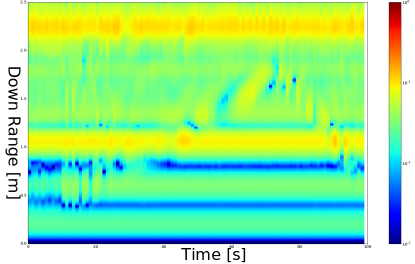
\includegraphics[max width=\linewidth]{figures/walabot_disttest}
        \caption{Range profile (\textit{y-axis}) over time (\textit{x-axis}) while the robot was moved at constant speed away and towards the Walabot sensor}
        \label{fig:walabot_dynamic_data}
    \end{subfigure}%
    \caption{Dynamic range test with the Walabot sensor}
\end{figure}

The figure shows that the Walabot has problems with what looks like
standing waves. The great amount of background signal is also visible.
Because of its static nature, this can easily removed for a fixed radar.
As some Walabot reviewers have noticed \cite{Valens2016} this background
signal changes heavily and seemingly random when the sensor is moved.
This makes the signal processing very difficult.

Walabot advertises object detection capabilities. The catch with this
mode is however that the number of objects to be detected must be
configured as a fixed parameter first.

\subsubsection{Omniradar RIC60-A}\label{omniradar}

With its good range resolution and a good idea of its capabilities from \cite{Ernst2016}, this sensor promised good results. It will provide the basis for the proof of concept implementation, so it receives a more detailed look.

Founded in 2010, Omniradar\footnote{\url{https://www.omniradar.com/}} is a Dutch
startup\footnote{\url{https://www.crunchbase.com/organization/omniradar}} that
claims to be the first to integrate a complete \SI{60}{GHz} radar including
antennas and analog to digital conversion in one chip.

With the RIC60-A they offer a Radar Development Kit (RDK) that gives
\SI{7}{GHz} of bandwidth on two receiving antennas. An Altera Cyclone IV FPGA
handles the signal acquisition and communication. \Cref{fig:slide_RIC60A} shows the
radar IC and how the three antennas are integrated in silicon.

\begin{figure}[htbp]
    \centering
    \def\svgwidth{12cm}
    \input{gfx/pictures/slide_RIC60A.pdf_tex}
    \caption{Decapped Omniradar IC (top left); five cent coin as size reference (top right); schematic with antenna locations (botto left); and antenna directionality pattern of Omniradar's RIC60-A (bottom right). Adapted from \cite{Brouwer2015} p.9}
    \label{fig:slide_RIC60A}
\end{figure}

The radar sensor's beam is fan shaped, which means it is fairly
sensitive over a wide angle in azimuth direction, but relatively focused
in elevation. This makes it a very good candidate for the radar
reprojection, as targets can be seen from the robot in a wide field of
view, but floor and ceiling reflections are kept at a minimum. Of course
the sensor can also be rotated. Omniradar also supplies a horn-like
extension for the sensor board, which forms the radar sensitivity into a
pencil-shaped beam that is very focused at a narrow field of view.

\begin{figure}[htbp]
    \centering
    \begin{subfigure}[t]{0.51206961048\textwidth}
        \label{fig:omniradar}
        \includegraphics[max width=\linewidth]{pictures/omniradar}
        \caption{Omniradar's RIC60-A sensor with horn antenna extension, attached to the 3D-printed Kobuki mount}
    \end{subfigure}
    \hfill
    \begin{subfigure}[t]{0.43793038951\textwidth}
        \centering
        \label{fig:mount}
        \includegraphics[max width=\linewidth]{models/mount.png}
        \caption{3D model of the radar sensor mount, designed with OpenSCAD.}
    \end{subfigure}
    \caption{Radar sensor on mount and model of the mount.}
\end{figure}


\subparagraph{Radar mount}\label{radar-mount}

A 3D-printed part makes sure that the radar sensor is firmly mounted on
the robot as it explores its environment. The part was designed in
OpenSCAD\footnote{\url{http://www.openscad.org/}} and printed on a
Dremel 3D printer\footnote{\url{https://3dprinter.dremel.com/}}. The bottom
mount hole positions were extracted from the mechanical drawings of the
Kobuki Base \cite{YujinRobot2012}; the side holes from the Altium layer
document of the version 3.2 Omniradar interface board
\cite{Omniradar2014}.

When rotated to face to the left side of the robot, the RPLidar mount
was in the way, so parts of the print had to be clipped off.

Two screws hold the Omniradar interface board to the mount. The other
two mounting holes in the interface board hold the Omniradar sensor
board. The horn extension can be affixed to these screws as well. If a
different sensor orientation is necessary, the sensor board can be
rotated by \ang{90}, thanks to the symmetric layout.

\subparagraph{Doppler sensitivity}\label{doppler-sensitivity}

The Omniradar FMCW radar is not sensitive enough to use the Doppler
speed directly. The following example illustrates this.

The RIC60A has a sensitivity of \SI{400}{Hz\per(m/s)}. A target with a
doppler speed of \SI{0.02}{m\per s} (A low speed at which the Kobuki robot
still moves continuously and without jerking) will cause a frequency
spike with a shift of \(\SI{8}{Hz}\) in the FMCW beat frequency.

The speed resolution capability is inversely proportional to the
measurement or acquisition time. A \SI{10}{ms} long acquisition gives a \SI{100}{Hz}
frequency resolution, or a speed resolution of \SI{0.9}{km/h} (or \SI{0.25}{m/s}).

Sampling frequency \(F_s=\SI{25}{MHz}\) and RIC60A Doppler sensitivity,
\(S_D = \SI{400}{Hz\per(m/s)}\) are constant values of the Omniradar RDK.

Given a chirp duration of \(T_{chirp} = \SI{2.5}{ms}\), we get
\(N_s = t_{chirp} F_s = 62500\) Samples,
\(N_r = \lfloor \frac{N_s}{2} \rfloor = 31250\) Samples per
up/downsweep, \(dF = \frac{F_s}{N_r - 1} = \SI{800}{Hz}\) FFT frequency bin
width and hence a Doppler resolution of \(\frac{dF}{S_D} = \SI{2}{m/s}\).

Even with subsample peak interpolation the accuracy will not be very
good and targets will be reprojected at imprecise angles.

It would be possible to use higher precision equipment. But another
solution is to track the movement of target peaks in the range profile,
using the Peak Gradient algorithm.

TODO wording?

\subsection{Optimal chirp time configuration}\label{optimal-chirp-time-configuration}

The chirp duration \(t_{chirp}\) is configurable and has an effect on
how the raw range profile data will look like.

\textbf{Very short durations} (\(<\SI{2}{ms}\)) incur a considerable processing
overhead to acquisition time ratio and have a very low SNR.\\
\textbf{Short durations} (\(<\SI{5}{ms}\)) have acceptable SNR, and are more
efficient with respect to overhead.\\
\textbf{Long durations} (\(>\SI{15}{ms}\))
have good SNR, and don't create a lot of overhead. However at higher
robot speeds, target peaks get blurred over several range bins as they
move in range. Less intense target echos are more difficult to detect
then.\\
\textbf{Very long durations} (\(>\SI{20}{ms}\)) required the Omniradar
driver to be patched on Linux so as not to freeze when chirps longer
than \SI{20}{ms} are requested. Even with the patched driver the RDK's FPGA
firmware is not very reliable at sending large volumes of data at once
and corrupts packet headers or aborts transmissions intermittently.

The optimal range was empirically found to lie between \SI{2}{ms} and \SI{10}{ms}.

TODO wording here

\Cref{fig:fig_chirp_eff} shows the chirp efficiency
\(\eta = \frac{n_{chirp}~t_{chirp}}{t_{msg}}\), with number of
consecutive sweeps \(n_{chirp}\) (two in the graph's data source), chirp
length \(t_{chirp}\), and \(t_{msg}\) the time since last radar message.

\begin{figure}[htbp]
    \centering
    \def\svgwidth{10cm}
    \input{gfx/fig_svg/chirp_eff.pdf_tex}
    \caption{Chirp efficiency \(\eta\) (measurement time per time spent) for various chirp lengths}
    \label{fig:fig_chirp_eff}
\end{figure}

The chirp length has an effect on accuracy and resolution. \Cref{fig:fig_compare_chirp_times} shows the range profiles of one scene, recorded over \SI{10}{s}. Short chirp times lead to a higher noise floor, but exhibit less variance, i.e. a slimmer band of frequencies. Longer measurement times have a lower noise floor but have more outliers. Especially with the horn extension attached longer measurement time also improves SNR.

\begin{figure}[htbp]
    \centering
    \begin{subfigure}{0.475 \textwidth}
        \centering
        \def\svgwidth{\linewidth} \small
        \input{gfx/fig_svg/chirp_comp_2.pdf_tex}
        \caption{Normalized echo intensity of range profiles without horn extension}
        \bigskip
    \end{subfigure}
    \hfill
    \begin{subfigure}{0.475 \textwidth}
        \centering
        \def\svgwidth{\linewidth} \small
        \input{gfx/fig_svg/chirp_comp_1.pdf_tex}
        \caption{Normalized echo intensity of range profiles with horn extension}
        \bigskip
    \end{subfigure}
    \begin{subfigure}{0.475 \textwidth}
        \centering
        \def\svgwidth{\linewidth} \small
        \input{gfx/fig_svg/chirp_comp_4.pdf_tex}
        \caption{Normalized harmonic mean of range profiles, without horn extension}
    \end{subfigure}
    \hfill
    \begin{subfigure}{0.475 \textwidth}
        \centering
        \def\svgwidth{\linewidth} \small
        \input{gfx/fig_svg/chirp_comp_3.pdf_tex}
        \caption{Normalized harmonic mean of range profiles, with horn extension}
    \end{subfigure}
    \caption{Effect of chirp length on SNR; with and without Horn extension}
    \label{fig:fig_compare_chirp_times}
\end{figure}
